\section{Node.js}
\label{ch:nodejs}

\subsection{Présentation}

Node.js est une plateforme open source pour le développement d’application coté serveur.

Il a été créé par Ryan Dahi en février 2009 et est depuis devenu très populaire. L’esprit de Node est similaire à Twisted pour Python et Eventmachine pour Ruby.

Il se compose délibérément d’une bibliothèque de base minimaliste accompagné d’un écosystème riche. Il fonctionne au dessus du moteur V8.  V8 est un moteur JavaScript très rapide développé par les ingénieurs de chez Google.

Le moteur JavaScript V8 de Google utilisé dans Chrome fait partie des moteurs JavaScript les plus puissants du marché.

JavaScript est populaire coté client, mais depuis peu il est un langage plébiscité pour le développement coté serveur.

Node permet de développer très simplement des applications scalables. : l'idée est d'utiliser des IO non bloquantes pour gérer toutes les requêtes entrantes, sortantes ainsi que tout le processus lié à la requête.




La page d’acceuil de Node.js le décrit ainsi:

“Node.js est une plateforme construire sur le moteur JavaScript de Chrome pour construire facilement des applications réseau rapides et évolutives. Node.js utilise une gestion d'événement basé sur des I/O non bloquantes, qui le rend léger et efficace, idéal pour les applications de données intensives en temps réels qui s’éxécutent à travers des dispositifs distribués. http://nodejs.org

Cela peut sembler énigmatique aux nouveaux arrivants, mais il résume succinctement certaines principales forces de Node.js et mérite d'être explorée plus en détail. Les gens sont souvent surpris quand ils entendent que JavaScript est un vrai langage de programmation complet et entier. Pour la communauté des développeurs, JavaScript n’est pas un vrai langage comme C, C++ ou Java.

Depuis ses humbles débuts, JavaScript a évolué et est désormais pris en charge dans tout les principaux navigateurs, y compris ceux sur les appareils mobiles. non seulement il est un langage populaire, mais les outils et frameworks actuellement disponibles sont nombreux et efficace, il est reconnu comme un langage puissant. JavaScript en tant que plateforme de développement coté serveur prend en charge l’intégration continue, le déploiement continu, les connexions aux bases de données relations, les architectures orientés services  et à peu prêt toutes les techniques disponibles.

En conjonction avec le moteur JavaScript V8 de Google, il est maintenant extrêmement rapide. En fait il est plusieurs fois plus rapide que les autres langages de script comme Ruby et Python. Contre Python 3, le moteur JavaScript V8 est environ 13 fois plus rapide avec un code similaire. Node.js est plus rapide d’environ 8 fois que Ruby 1.9. Ce sont des points de repère incroyable pour un langage dynamique, et est dû en grande partie à des optimisations du moteur v8.

La description officielle des discussions sur le modèle événementiel à I/O on bloquant est le suivant: Traditionnellement, la programmation se fait de manière synchrone: une ligne de commande est exécuté, le système attend le résultat, le résultat est traité, puis l’exécution reprend.

Parfois, attendre le résultat peut reprendre après un certain temps, par exemple, la lecture d’une base de données ou d’écriture sur un réseau.

Dans des langages tels que Java et C\#, une solution consiste à lancer un nouveau thread. Un thread peut être considéré comme un processus léger qui exécute des taches. Programmer en utilisant des thread peut être difficile parce que plusieurs thread peuvent essayer d’accéder simultanément à la même ressource. Sans disséquer les subtilités de la programmation multi-threading, vous pouvez imaginer que ce serait désastreux pour un thread à incrémenter alors qu’un autre thread décrémente le compteur en même temps.



\subsection{Architecture de Node.js}

\begin{center}
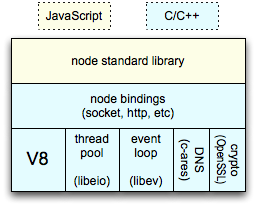
\includegraphics[scale=1]{img/nodejsarch.png}
\label{Graphique technologie node.js}
\end{center}

Node.js est en grande partie écrit en C/C++.
Mais il possède un framework complet en JavaScript pour développer nos applications. C'est ce qui le rend particulièrement intéressant.

\subsection{Boucle d’évènement}

Node est écrit en C++ et utilisant la bibliothèque libev de Marc Lehman, la boucle d’évenement utilise epoll ou kqueue comme mécanisme d’évenement évolutifs.

\subsection{I/O non bloquant}

Node évite de perdre en temps de calcul CPU habituellement rencontré par l’attente d’une réponse d’entrée ou de sortie (base de données, système de fichier, service web, …) grâce à l’asynchrone complet fourni par la bibliothèque libeiode Marc Lehmann 

Ces caractéristiques  permettent à Node de gérer une grande quantité de trafic en manipulant le plus rapidement une demande afin de libérer le thread pour la demande suivante. Node.js est un serveur capable de répondre au problème C10K.

Node possède un support intégré de la plupart des protocoles importants comme TCP, DNS et HTTP (celui qui nous interesse ici). L’objectif de la conception d’une application Node est que toute fonction effectue une E / S doit utiliser un callback. C’est pourquoi il n’existe pas de méthode de blocage prévu dans l’API de Node.

\subsection{Asynchrone}

Prenons l'exemple du serveur Apache. Chaque requête HTTP entrante se voit allouer un thread. Celui-ci est utilisé pendant toute la durée du traitement de la requête : lecture/écriture en base de données, lecture/écriture dans des fichiers de logs ou autres, exécution de code... Ainsi, si votre code côté serveur fait un accès à la base de données, celui-ci est en attente de la réponse. De plus, durant toute la durée de la requête, le client sera bloqué, en attente de la réponse du serveur.

Node et plus globalement les serveurs dits non bloquants (comme Netty ou Deft pour ceux qui tournent sur JVM) adoptent une autre approche. Node n'utilise qu'un seul thread pour gérer les requêtes entrantes. De plus, Node ne propose pas, dans ses API, de fonctions bloquantes. Ainsi, tout notre code est asynchrone. L'avantage immédiat à cela est la simplification à l'extrême de la gestion de la concurrence dans nos applications qui n'est ici plus gérée par le développeur mais directement par l'OS.

Concrètement, toutes les fonctions fournies par Node prennent en paramètre un callback. Une fois que la fonction termine son traitement, le callback sera appelé avec le résultat en paramètre et une éventuelle erreur. Ainsi, pendant toute la durée du traitement, le thread est relâché et peut être donné à une autre requête pour effectuer un autre traitement. Nous sommes donc face à un système évènementiel. Et Javascript est un très bon choix de langage du fait que l'on peut programmer de manière fonctionnelle avec celui-ci. Les callbacks dans tous les sens sont bien connu avec l’utilisation de librairies comme jQuery qui nous habituent depuis déjà quelques temps à ce type de développement.

\subsection{Performance}

Node.js est rapide. L'une des critiques les plus fréquentes à propos des langages interprétés comme PHP, Python et Ruby est la performance. Jason Hoffman, directeur de la technologie de Joyent, a discuté de la façon dont Node.js est ultra performant et peut être ralenti à cause des systèmes d'exploitation. Un seul core avec moins de 1 Go de RAM est capable de gérer 10 Go de trafic et un million de terminaux connectés. La combinaison de 24 d'entre eux sur une seule machine produit un niveau global de débit qui dépasse les capacité des systèmes d'exploitation et Piles TCP / IP. En d'autres termes, avec une application bien conçue, ce n'est pas Node.js le goulot d'étranglement c'est votre système d'exploitation.

\subsection{Communauté}

Malgré sa jeunesse, la communauté Node grandis de plus en plus rapidement et le dépot de Node est le 3ème dépot le plus suivi sur Github.

\subsection{Forces}

\begin{list}{•}{}
  \item
  Bien que Node.js date seulement de 2009 :
    \begin{list}{•}{}
      \item
      il a déjà un bon système de package : Node Package Manager que la grande majorité de la communauté semble utiliser
      \item
          il a déjà une très forte communauté, de très nombreuses librairies, exemple : plein de librairie classées, déjà plus de 9000 packages sur npm
      \item
      de plus en plus de sociétés semblent l'utiliser comme Linkendin par exemple.
    \end{list}
    
    
  \item 
  tous les développeurs web (front-end) connaissent le langage, il est très populaire. Par conséquent, pour passer à Node.js il n'y a pas le frein d'apprendre un nouveau langage comme ça serait le cas avec l'utilisation d'un framework web basé sur Ruby ou Python. Je pense que dans les mois qui viennent, de nombreux développeurs PHP vont passer à Node.js… surtout ceux qui regardaient ailleurs mais qui ne souhaitent pas apprendre un nouveau langage.

  \item
      la possibilité de partager du code (librairies communes…) entre la partie client et serveur peut être intéressant. La question se pose de plus en plus étant donnée qu'on est de plus en plus amené à effectuer beaucoup de traitement coté client (exemple avec Backbone.js).
      
  \item
  Ces derniers jours, la visualisation de screencast sur le framework JavaScript Meteor m'a profondément intéressé.
  
  \item
  Autre exemple, il est possible d'utiliser la même API Canvas coté client et coté serveur (avec node-canvas).
  
  \item
  Node.js semble être très rapide, ça tient très bien la monté en charge.
  
  \item
  La vitesse de l'interpréteur Javascript est en constante progression V8.

\end{list}

\subsection{Retour d'expérience Linkedin}